%%%%%%%%%%%%%%%%%%%%%%%%%%%%%%%%%%%%%%%%%%%%
\chapter{Classification and Regression Analysis}
%%%%%%%%%%%%%%%%%%%%%%%%%%%%%%%%%%%%%%%%%%%%
\begin{center}
  \begin{minipage}{0.75\textwidth}
    \begin{small}
      “...in the whole of nature there is something which makes all things, so too is it in the soul.”\\
      \null\hfill\emph{On the Soul, The Philosopher}
    \end{small}
  \end{minipage}
  \vspace{0.5cm}
\end{center}

\section{Support Vector Machines}
A Support Vector Machine (SVM) is binary classification tool that is used in machine learning classification and regression problems.  SVMs attempt to separate data by creating a hyper plane that maximizes the distance between each of the classes.  This is often performed in high dimensional spaces, where each sample is described by multiple features.

The python package Sci-Kit Learn provides access to SVM modules and utilities that make it easy to run analysis on datasets.  This packages allows for easily performing machine learning classification and cross validation.  Pipelines are useful for streamlining any preprocessing steps before classification.  This allows for easy modification and testing of various steps in the machine learning process.  A pipeline can be setup in order to allow for easy access to the classifier processing steps during analysis such as,
%
\begin{lstlisting}
from sklearn import svm
from sklearn.multiclass import OneVsRestClassifier
from sklearn.preprocessing import StandardScaler

clf = OneVsRestClassifier(make_pipeline(
	StandardScaler(),
	svm.SVC(kernel='linear', probability=True)))

\end{lstlisting}
%
The OneVsRestClassifier was used to extend binary classification methods to multiclass problems, allowing for the use of SVC to classify Red Oak, American Ash and Sugar Maple leaves.  The chosen kernel was linear.  The GridSearch module of sklearn can additionally be utilized to find the most optimal parameters for fitting the data, when free parameters are available.

In Support vector classification, the C and epsilon are tunable parameters [TODO explain these parameters and processes for finding right values of them].
%%%%%%%%%%%%%%%%%%%%%%%%%%%%%%%%%%%%%%%%%%%%%%%%%%%%%%%%%%%%%%%%%%%%%
\subsection{Validation of Classifier Results}
%%%%%%%%%%%%%%%%%%%%%%%%%%%%%%%%%%%%%%%%%%%%%%%%%%%%%%%%%%%%%%%%%%%%%
Cross validation of results is important for reducing the training and testing bias inherent to some datasets.  Learning curves are useful visualization tools for showing how adding more samples to a testing set affects the classification score or ability.

A stratified K-fold validation can be used for ensuring that when sets of training and testing sets are created, the testing sets contain equal amounts of each class.  This is especially useful in unequally distributed sets of data.

In binary classification problems, it is of interest to understand the ability of a classifier to correctly predict the true condition of the sample under inspection.  The possible outcomes of a classification can be found in Figure
\begin{figure}
    \begin{center}
        \makebox[\textwidth]{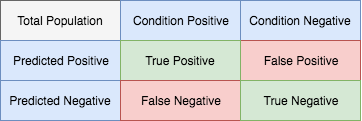
\includegraphics[scale=0.6]{/Sources/Classification_Regression/ROC.png}}
    \end{center}
    \caption{Receiver Operating Characteristic Outcomes}
    \label{fig:polarization}
\end{figure}
A true positive result is one that correctly identifies the sample.  False negatives incorrectly predict that a sample was not in its own class.  False positives are when samples are incorrectly identified with another class.  True negatives correctly identify that a sample is not a member of the class being tested against.   These rates can be combined into useful metrics for quantifying a classifiers performance.

The precision of a classifier is a measure of the relevancy of its results.  It is an overall indicator of the false positive rate of a classifier.
%
\begin{align}
    P = \frac{T_p}{T_p + F_p}
\end{align}
%
were $T_p$ is the number of true positives and $F_p$ is the number of false positives that result from testing on the trained classifier.  The recall, also known as the sensitivity, is defined as
%
\begin{align}
    R = \frac{T_p}{T_p + F_p}
\end{align}
%
and tells the amount of relevant samples returned and $F_n$ is the false negative rate.  The F1 score is the harmonic mean between the precision and recall, and is defined as
%
\begin{align}
    F1 = 2\frac{PR}{P + R}
\end{align}
%
The classification report shows a useful cross validated summary of the precision, recall, F1 score, and support vectors that result from testing different dataset.

All of these features are available in the Sklearn package and an example is shown below.
%
\begin{lstlisting}
from sklearn.model_selection import classification_report, StratifiedKFold

cv = StratifiedKFold(5, shuffle=True)

for train, test in cv.split(X, y):
    y_test = label_binarize(y[test], classes=[0,1,2])

    fit = clf.fit(X[train], y[train])

    y_pred = fit.predict(X[test])

    print classification_report(y[test], y_pred)
\end{lstlisting}
%
These metrics are often visualized using receiver operating characteristic (ROC) curves for binary classification, and confusion matrices for multiclass problems.  ROC curves show the sensitivity vs the specificity [TODO explain specifity] of a binary classifier by plotting the false positive rate versus the true positive rate.  It “is a graphical plot that illustrates the diagnostic ability of a binary classifier system as its discrimination threshold is varied” [wiki]. The area under the ROC curve, often denoted AUC, is a measure equivalent to the score of a classifier. It should be noted that for multi-class problems ROC curves can be more optimistic than the individual performance metrics.

ROCs can be extended to multi-class problems, by using a one verse many techniques [TODO explain these techniques used] although a confusion matrix is often used to show the accuracy of a classifier between each of the various classes.  A confusion matrix shows the classifier score against each combination of true value and predicted value.  It therefore shows all outcomes of classification.

It is important to understand the bias and variance of a model when determining its overall effectiveness.  The bias is the average error for different training sets while the variance indicates how sensitive a model is to varying training sets.

Learning curves are a useful visualization tool for understanding the bias and variance of a classification model.  It is useful for determining if a model gets better at classifying samples, as the number of training samples increases.  If the score of a classifier decreases as the number of samples increases, the model has a high amount of bias.  The model performance is not generalized enough to handle more training data.  If, as the number of training samples increases, the score increases, the model could benefit from more training data.  If the score remains constant as the training samples increase, the model has low bias.

\section{Linear Regression}
A linear regression is a simple approach to supervised learning that has long been in use in the field of statistical learning.  It provides the ability to predict a quantitative response $Y$, given a predictor variable $X$.  The assumption when using this technique is that the relationship between these two variables is linear.  In general the form of a Simple Linear Regression is
%
\begin{align}
    Y = \beta_0 + \beta_1 X
\end{align}
%
where $\beta_0$ and $\beta_1$ are parameters that are calculated using a set of training data.  Once trained, this model can predict future output values for a given input.  When given a set of observations $\beta_0$ and $\beta_1$ are set in order to have a closeness between the predicted line and the actual observed data.  A common measure of this closeness is the least squares error.

The residual, $e$, for a given set of observations and predications is calculated
%
\begin{align}
    e_i = y_i - \hat{y_i}
\end{align}
%
These residuals can be used to calculate the Residual Sum of Squares \(RSS\), or the amount of variation left unexplained after performing the regression.  It is
\begin{align}
    RSS = {e_1}^2 + {e_2}^2 + \cdots\ + {e_n}^2
\end{align}
where $n$ is the number of observations in a dataset.

The Total Sum of Squares is the measure of how much variability exists within the data before the regression has been performed.  It is defined as
\begin{align}
    TSS = \sum_{i=0}^n (y_i - \bar{y})^2
\end{align}
where $\bar{y}$ is the mean.  Using the $RSS$ and $TSS$ allows for determining the accuracy within the model by calculating the $R^2$.  The $R^2$ is the "proportion of variability in $Y$ that can be explained by $X$". It is defined as
\begin{align}
    R^2 = \frac{TSS - RSS}{TSS} = 1 - \frac{RSS}{TSS}
\end{align}

For a given application it is difficult to determine what a 'good' $R^2$ score is, although it has been noted that in biological applications there can be a great deal of unexplained variance, sometimes even less than 0.1 \cite{stats}.  In these experiments a linear regression was utilized to correlate the relative water content of the Devils Ivy plant leaves, with the first principal component derived from texture and polarization characteristics.  $R^2$ was used to gauge the accuracy of the results.

\subsection{Principal Component Analysis}
When a dataset has a large number of features, it becomes difficult to visualize these features against a given model.  Principal Component Analysis (PCA) allows for reducing the dimensionality of data by combining variables that are highly correlated. By performing this process, it becomes possible to observe only the features that contain as much information as possible.  For the dataset utilized in these experiments the features were more than a few dozen in total so reducing the dimensionality was important when visually interpreting the results. The Scikit-learn Python module has a helper utility to provide this reduction in dimensionality.  The code used for performing the linear regression and plotting the first principal component versus the relative water content can be found in Figure.
\newpage
\begin{lstlisting}
    from __future__ import division
    import numpy as np
    from sklearn.model_selection import train_test_split, cross_val_score
    from sklearn import linear_model
    from sklearn.decomposition import PCA as sklearnPCA
    import matplotlib.pyplot as plt
    from sklearn.preprocessing import normalize
    from sklearn.metrics import r2_score, explained_variance_score, mean_squared_error
    from sklearn.preprocessing import FunctionTransformer
    from sklearn.preprocessing import PolynomialFeatures

    transformer = FunctionTransformer(np.log1p)
    data = np.genfromtxt('data.csv', delimiter=',')
    X = data[:,1:]
    X = normalize(X, axis=1)
    X = transformer.transform(X)
    poly = PolynomialFeatures(degree=1)
    X = poly.fit_transform(X)
    y = data[:,0]

    pca = sklearnPCA(n_components=1)
    X = pca.fit_transform(X)

    mean = np.mean(X)
    std = np.std(X)

    X_train, X_test, y_train, y_test = train_test_split(X, y, test_size=0.2, random_state=4)
    regr = linear_model.LinearRegression()
    regr.fit(X, y)

    y_pred = regr.predict(X)

    print "r2: ", r2_score(y, y_pred, multioutput='variance_weighted')
    print "explained_variance_score: ", explained_variance_score(y, y_pred)
    print "root mean squared: ", mean_squared_error(y, y_pred)
    scores = cross_val_score(regr, X, y, cv=10)
    print("Accuracy: %0.2f (+/- %0.2f)" % (scores.mean(), scores.std() * 2))

    plt.title('Linear Regression For Relative Water Content')
    plt.xlabel('First Principal Component')
    plt.ylabel('Relative Water Content')
    plt.scatter(X[:,0], y)
    plt.plot(X[:,0].reshape(-1, 1), y_pred)

    plt.show()
\end{lstlisting}
